\documentclass{beamer}
\beamertemplatenavigationsymbolsempty 
\usepackage{minted}

\title{Detecting Asteroids with Neural Networks\\ using PyBrain}
%\author{Dustin Ingram}
\author{
    \texorpdfstring{
        Dustin Ingram\newline
        \texttt{\href{mailto:dustin@drexel.edu}{dustin@drexel.edu}}\newline
        di @ GitHub
    }{Author}
}
\institute{Philly Python Users Group}
\date{\today}

\begin{document}
\maketitle

\begin{frame}
    \frametitle{The goal}
    Build and train a neural network to correctly identify asteroids in
    astrophotography data, using \textbf{PyBrain}, a modular machine learning
    library for Python.
\end{frame}

\begin{frame}
    \frametitle{Disclaimer}
    \begin{itemize}
        \item I am not an expert;
        \item This is not (quite) my field;
        \item Some things might be wrong!
    \end{itemize}
\end{frame}

\begin{frame}
    \frametitle{The data}
    The Sloan Digital Sky Survey:
    \begin{itemize}
        \item "One of the most ambitious and influential surveys in the history
        of astronomy."
        \item Approx 35\% of sky;
        \item Largest uniform survey of the sky yet accomplished;
        \item Data is freely available online;
        \item Each image is 922x680 pixels.
    \end{itemize}
\end{frame}

{
    \usebackgroundtemplate{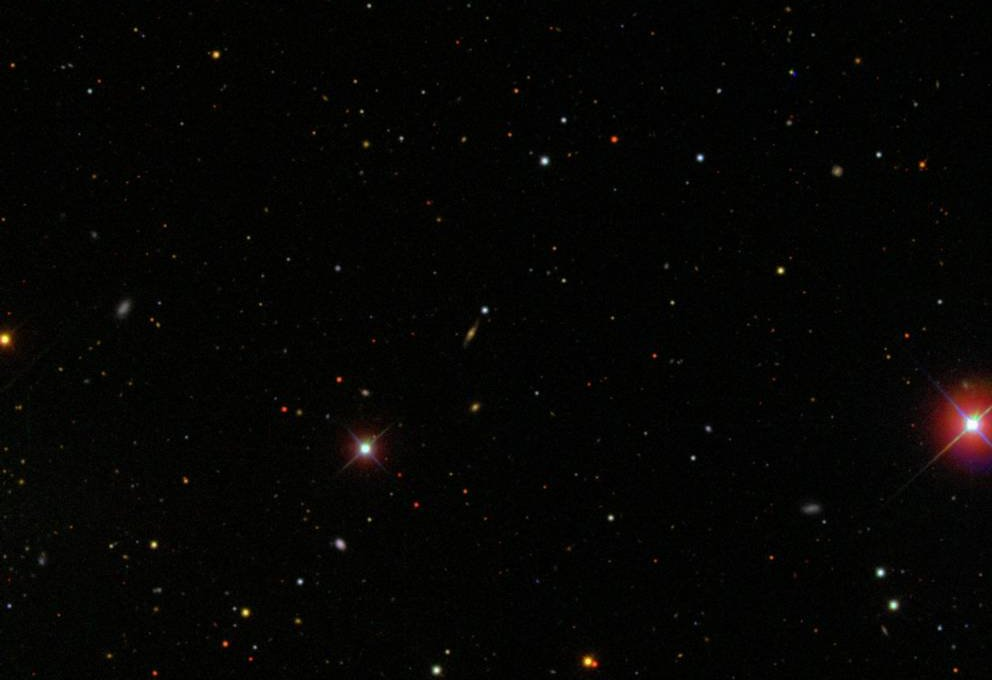
\includegraphics[width=\paperwidth,height=\paperheight]{18364_unbox.jpg}}
    \begin{frame}[plain] \end{frame}
}

{
    \usebackgroundtemplate{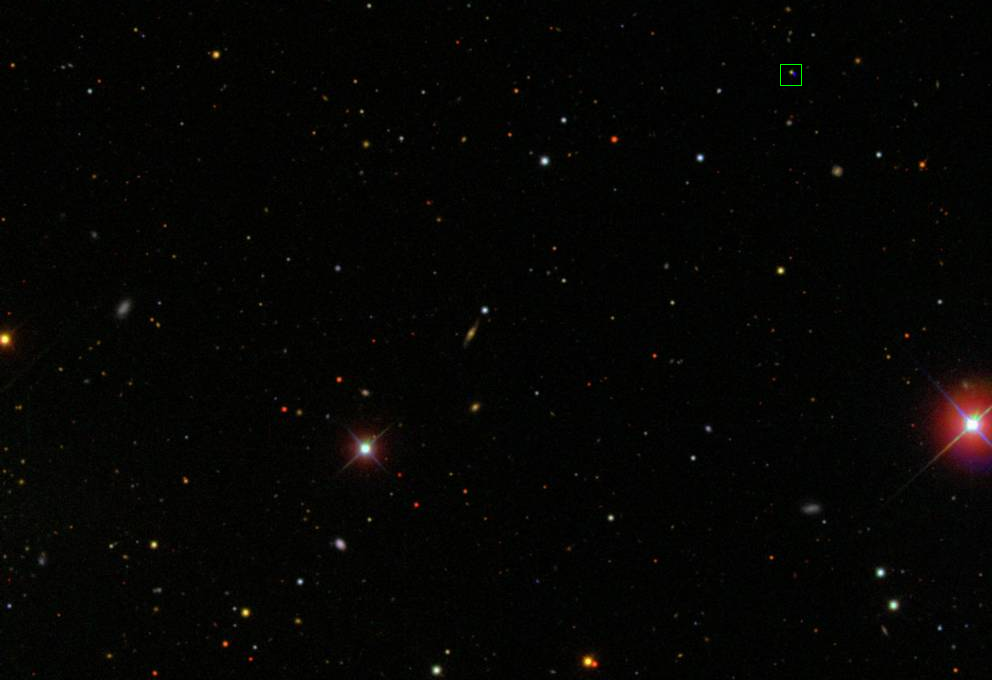
\includegraphics[width=\paperwidth,height=\paperheight]{18364_box.png}}
    \begin{frame}[plain] \end{frame}
}

\begin{frame}
    \frametitle{An example asteroid}
    \begin{figure}
        \centering
        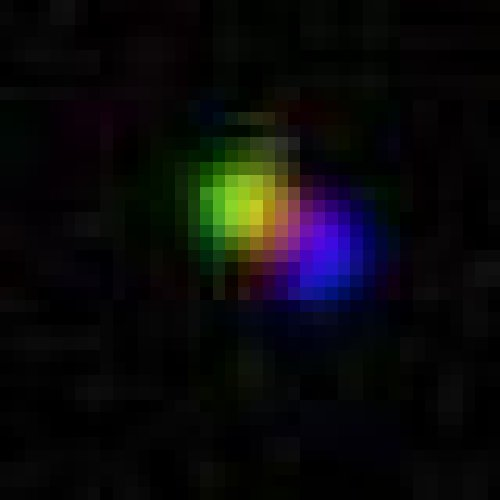
\includegraphics[height=0.8\paperheight]{18364_large.jpg}
    \end{figure}
\end{frame}

\begin{frame}
    \frametitle{Why use a Neural Network?}
    This type of classification is well suited for a neural network:
    \begin{itemize}
        \item We have a clear set of training data;
        \item There is a small amount of input features which can accurately
        define an item:
        \begin{itemize}
            \item Ratio valid hues to non-valid hues
            \item Best possible cluster collinearity
            \item Best possible average cluster distance
        \end{itemize}
        \item Each of the input features can be resolved to a $0\to 1$ metric;
        \item The output is either affirmative (1) or negative (0);
        \item Neural network activation will be fast!
    \end{itemize}
\end{frame}

\begin{frame}
    \frametitle{Getting started}
    Getting the initial training data:
    \begin{itemize}
        \item Small tool to extract potential candidates from full-scale images;
        \item Extremely na\"{\i}ve, approx 100:5 false positives to actual positives;
        \item Very low false negatives (approx 1:1000);
        \item Incredibly slow (complex scan of 100Ks of potentials);
        \item Manual classification, somewhat slow;
        \item Yields approx 250 valid items, 500 invalid items;
        \item Form is a set of 20x20px images.
    \end{itemize}
\end{frame}

\begin{frame}[fragile]
    \frametitle{Making the data set}
    \inputminted[firstline=2,lastline=2,linenos,frame=lines,firstnumber=2]{python}{brain.py}
    \inputminted[firstline=15,lastline=26,linenos,frame=lines,firstnumber=15]{python}{brain.py}
\end{frame}

\begin{frame}[fragile]
    \frametitle{Building and training the network}
    \inputminted[firstline=3,lastline=4,linenos,frame=lines,firstnumber=3]{python}{brain.py}
    \inputminted[firstline=29,lastline=40,linenos,frame=lines,firstnumber=29]{python}{brain.py}
\end{frame}

\begin{frame}
    \frametitle{Building the neural network}
    The resulting neural network:
    \begin{figure}
        \centering
        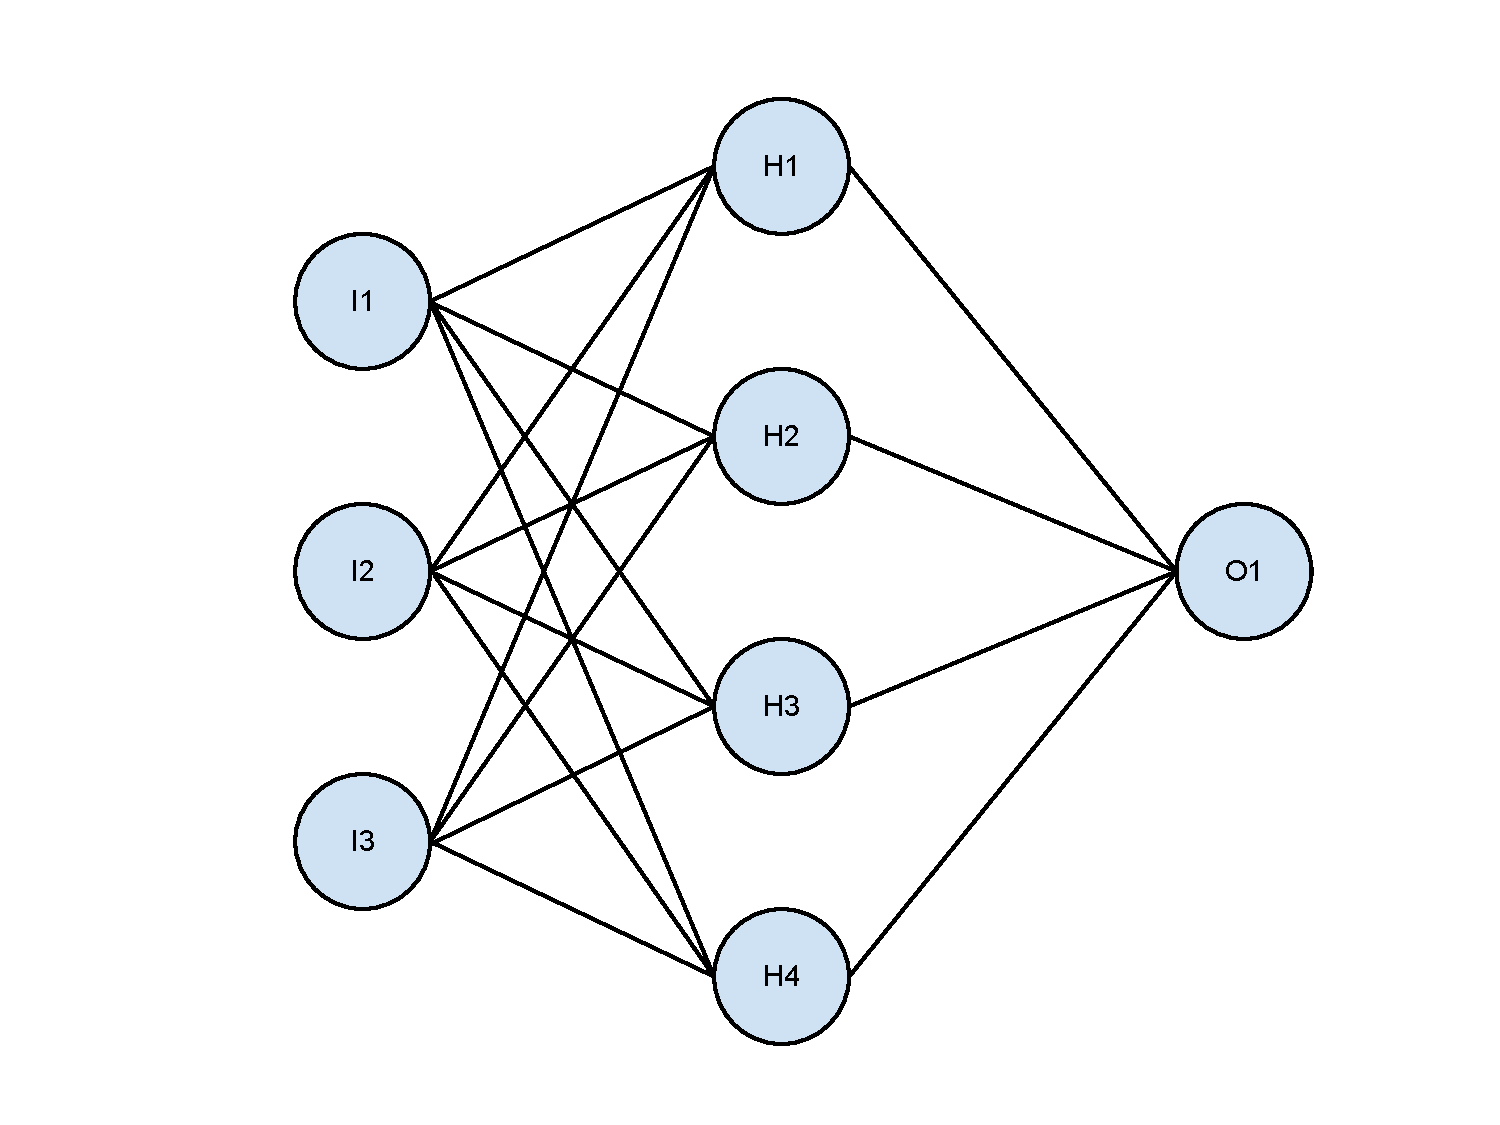
\includegraphics[height=0.8\paperheight]{nn.pdf}
    \end{figure}
\end{frame}

\begin{frame}
    \frametitle{Training the network}
    \begin{itemize}
        \item Approx 250 valid items;
        \item Approx 500 invalid items;
        \item Trained for 5,000 iterations;
        \item Took approx. 3 hours;
        \item Probably could have gotten by with less iterations.
    \end{itemize}
\end{frame}

\begin{frame}[fragile]
    \frametitle{Testing the network}
    \inputminted[firstline=9,lastline=10,linenos,frame=lines,firstnumber=9]{python}{brain.py}
    \inputminted[firstline=43,lastline=51,linenos,frame=lines,firstnumber=43]{python}{brain.py}
\end{frame}

\begin{frame}[fragile]
    \frametitle{Putting it all together}
    \inputminted[firstline=59,lastline=60,linenos,frame=lines,firstnumber=59,gobble=8]{python}{brain.py}
    \inputminted[firstline=66,lastline=67,linenos,frame=lines,firstnumber=66,gobble=4]{python}{brain.py}
\end{frame}

\begin{frame}
    \frametitle{Storing your neural network}
    \inputminted[firstline=8,lastline=8,linenos,frame=lines,firstnumber=8]{python}{brain.py}
    \inputminted[firstline=53,lastline=63,linenos,frame=lines,firstnumber=53]{python}{brain.py}
\end{frame}

\begin{frame}
    \begin{figure}
        \centering
        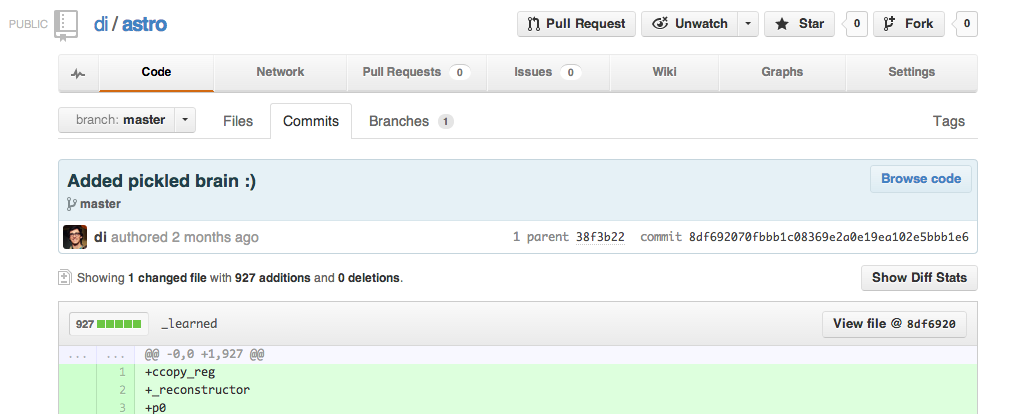
\includegraphics[height=\paperheight]{pickle.png}
    \end{figure}

\end{frame}

\begin{frame}
    \frametitle{Thanks!}
    \begin{itemize}
        \item Contact me:\\\texttt{\href{mailto:dustin@drexel.edu}{dustin@drexel.edu}}
        \item Source for this talk:\\ \url{https://github.com/di/astro}
        \item The Sloan Digital Sky Survey:\\ \url{http://www.sdss.org/}
        \item PyBrain:\\ \url{http://pybrain.org/}
    \end{itemize}
\end{frame}

\end{document}
